Model relacyjny zaprojektowany dla PostgreSQL oraz MySQL obejmuje dwanaście
tabel, podzielonych pod względem funkcjonalnym na trzy obszary: domenę
użytkownika i subskrypcji, domenę katalogu treści oraz domenę aktywności
użytkownika. Strukturę logiczną przedstawiono na rysunku~\ref{fig:schema_sql}.

\begin{figure}[H]
    \centering
    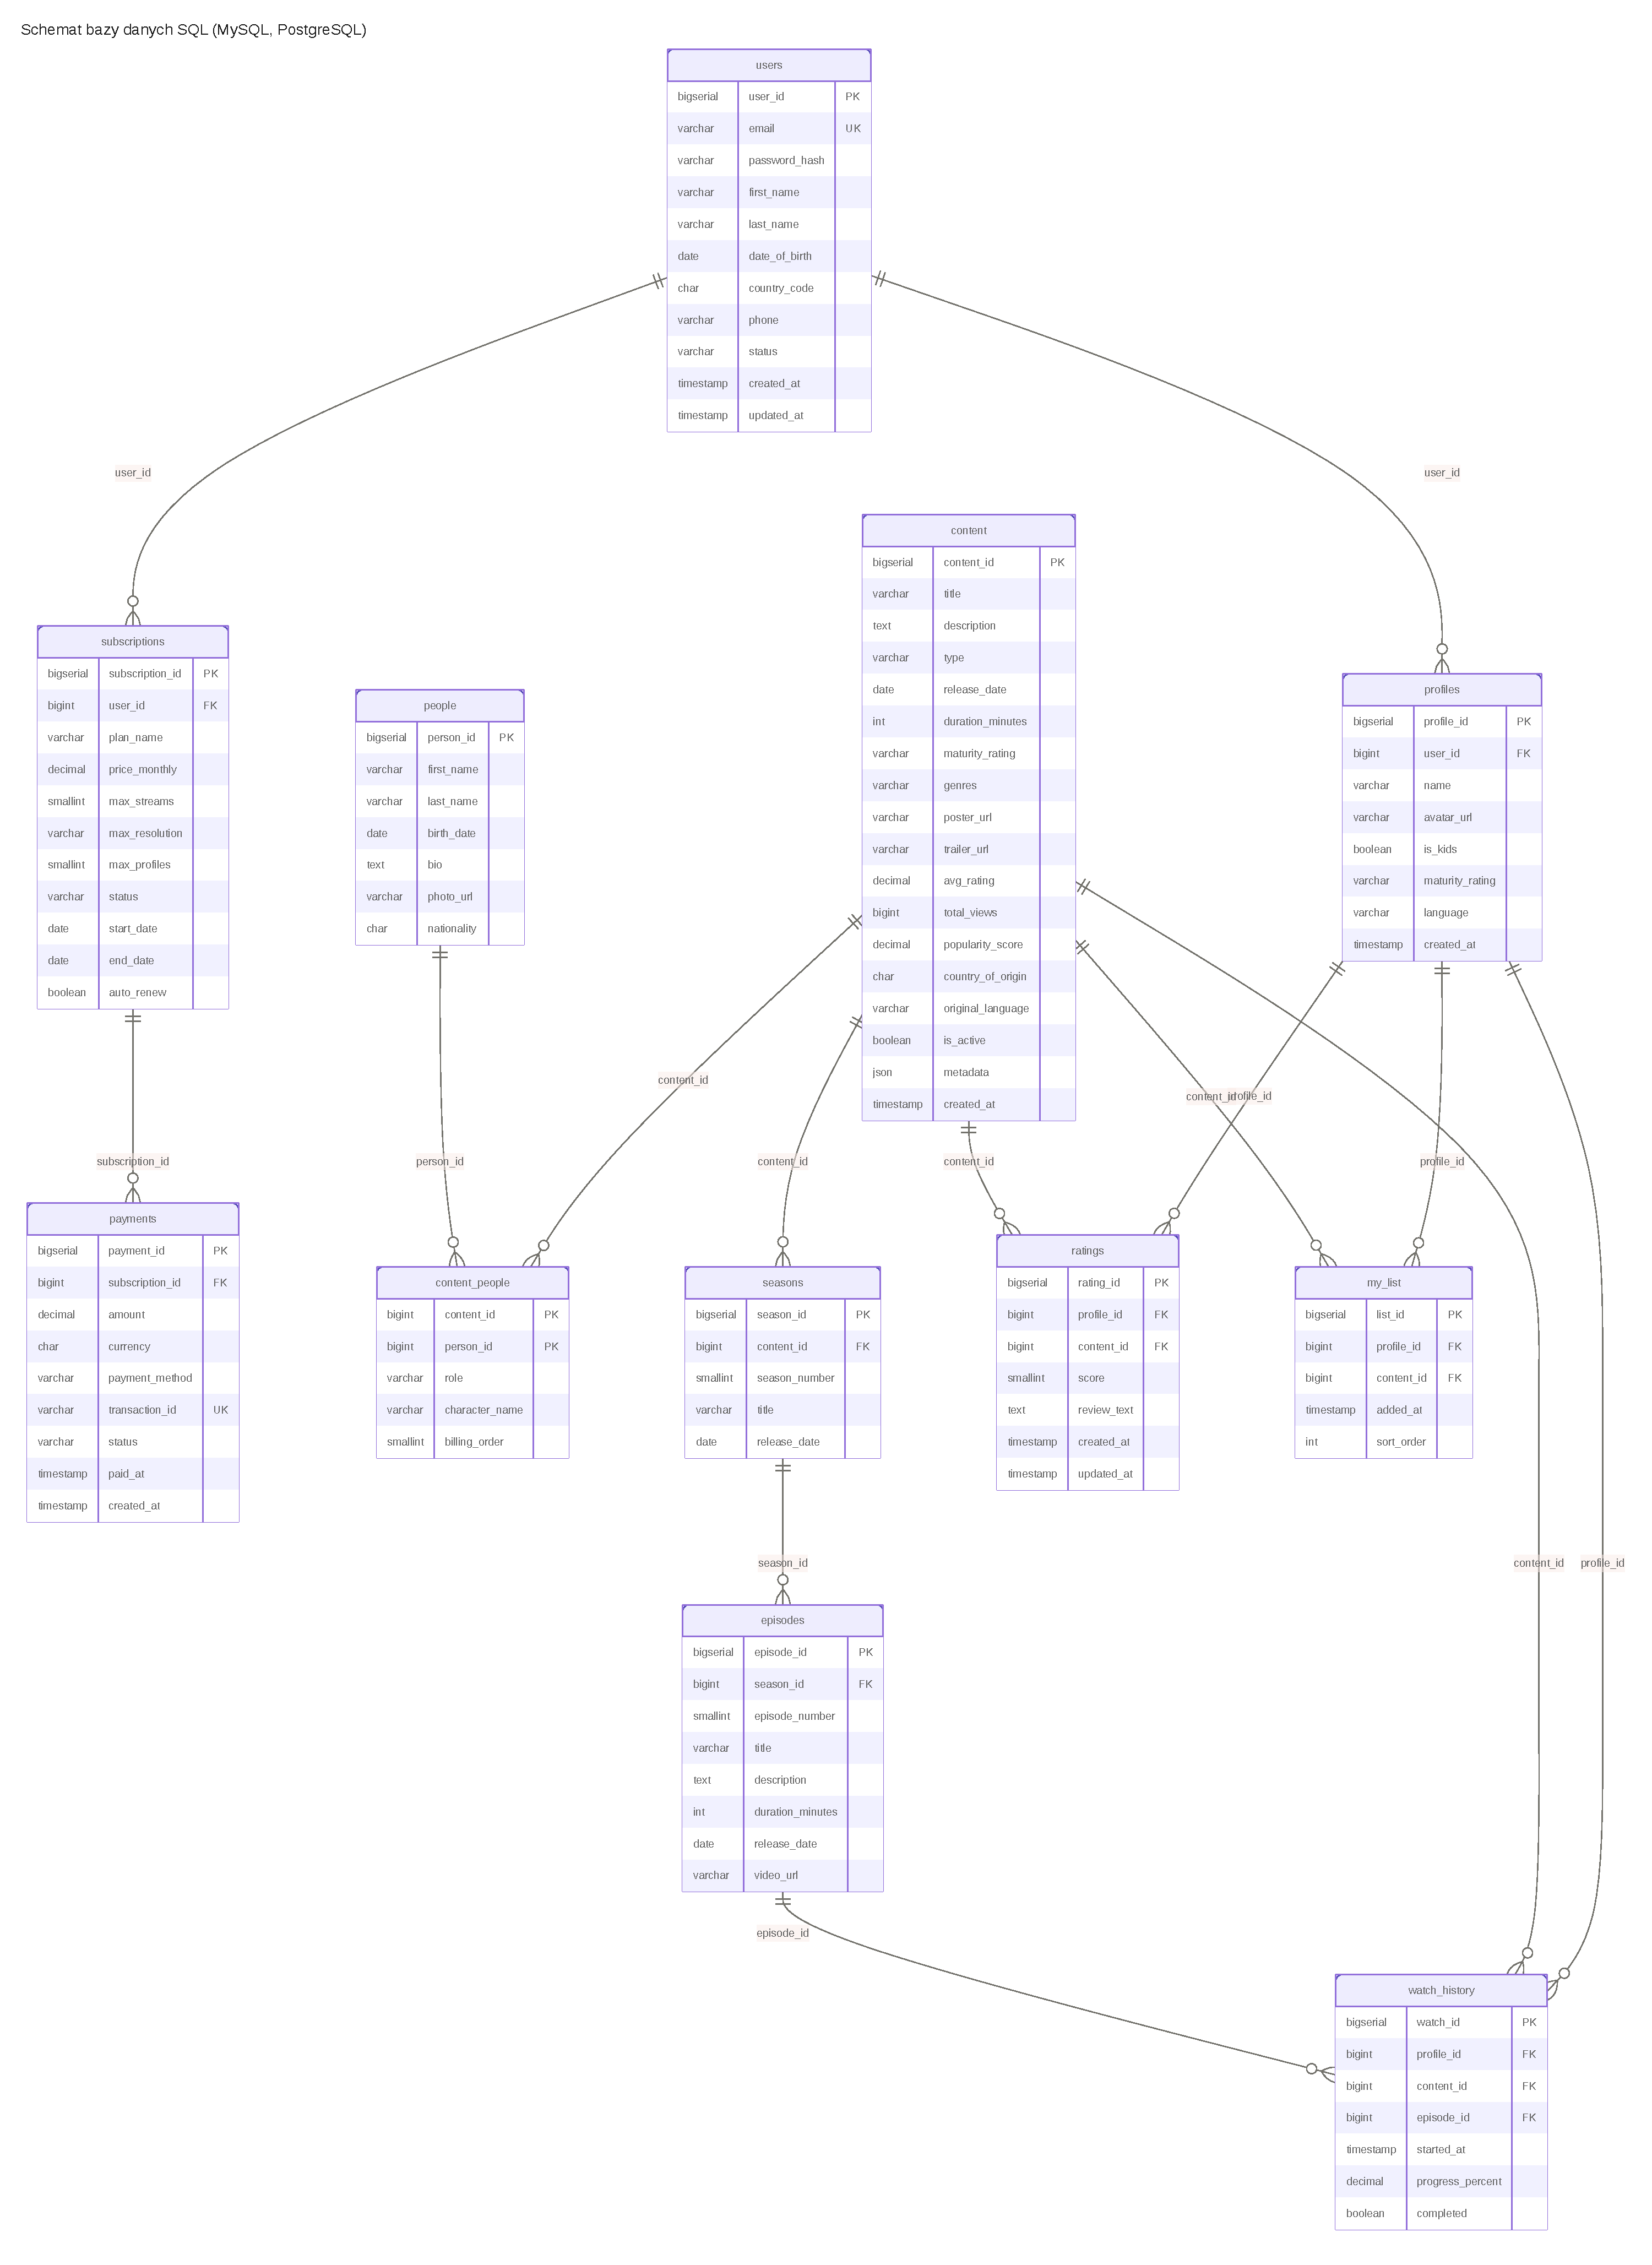
\includegraphics[width=1.0\textwidth]{charts/SchematBazy_SQL.pdf}
    \caption{Schemat relacyjny dla PostgreSQL oraz MySQL}
    \label{fig:schema_sql}
\end{figure}

Domena użytkownika reprezentowana jest przez tabelę \texttt{users}, w której
adres poczty elektronicznej posiada ograniczenie unikalności (\texttt{UNIQUE}),
oraz przez powiązaną z nią relacją jeden-do-wielu tabelę \texttt{profiles},
przechowującą dane poszczególnych profili w obrębie konta. Tabela
\texttt{subscriptions}, również powiązana z \texttt{users} relacją
jeden-do-wielu, rejestruje historię planów subskrypcyjnych wraz z ich
parametrami (cena, dopuszczalna liczba strumieni, maksymalna rozdzielczość).
Tabela \texttt{payments} zawiera informacje o pojedynczych transakcjach
płatniczych powiązanych z konkretną subskrypcją, przy czym pole
\texttt{transaction\_id} podlega ograniczeniu unikalności w celu
wyeliminowania duplikatów.

Domena katalogu treści jest zorganizowana wokół tabeli \texttt{content},
przechowującej zarówno filmy, jak i seriale, rozróżniane przez kolumnę
\texttt{type}. W przypadku seriali strukturę hierarchiczną odwzorowują
tabele \texttt{seasons} oraz \texttt{episodes}, połączone relacjami
jeden-do-wielu odpowiednio z \texttt{content} i \texttt{seasons}. Informacje
o osobach związanych z produkcją -- aktorach, reżyserach oraz scenarzystach --
są utrzymywane w tabeli \texttt{people}, natomiast ich powiązania z konkretnymi
tytułami modeluje tabela łącząca \texttt{content\_people}, realizująca
relację wiele-do-wielu. Klucz główny tej tabeli jest złożony z kolumn
\texttt{content\_id} oraz \texttt{person\_id}, a kolumna \texttt{role}
rozróżnia rodzaj uczestnictwa danej osoby (\textit{director}, \textit{writer},
\textit{actor}). Dla aktorów dodatkowe atrybuty obejmują nazwę odgrywanej
postaci (\texttt{character\_name}) oraz pozycję w napisach
(\texttt{billing\_order}). Gatunki treści zostały zdenormalizowane do postaci
listy w kolumnie \texttt{genres} typu \texttt{varchar}, co stanowi świadomy
kompromis pomiędzy normalizacją a wydajnością odczytu.

Domena aktywności użytkownika obejmuje trzy tabele rejestrujące interakcje
profilu z treścią. Tabela \texttt{watch\_history} przechowuje pojedyncze
sesje odtwarzania wraz z procentowym postępem (\texttt{progress\_percent})
oraz znacznikiem ukończenia (\texttt{completed}); klucze obce wskazują na
\texttt{profiles}, \texttt{content} oraz opcjonalnie \texttt{episodes}
w przypadku seriali. Tabela \texttt{ratings} zawiera oceny treści wystawione
przez profile, w skali liczbowej z możliwą dodatkową recenzją tekstową.
Tabela \texttt{my\_list} reprezentuje listę treści dodanych przez profil
do oglądania w przyszłości, z atrybutem \texttt{sort\_order} określającym
kolejność prezentacji.

Klucze główne wszystkich tabel zostały zaimplementowane jako wartości typu
\texttt{bigserial} (PostgreSQL) lub \texttt{BIGINT AUTO\_INCREMENT} (MySQL),
co zapewnia jednoznaczną identyfikację rekordów oraz monotonicznie rosnącą
sekwencję ułatwiającą wstawianie do indeksów typu B-tree. Klucze obce
zostały opatrzone ograniczeniami referencyjnymi gwarantującymi spójność
danych pomiędzy tabelami. Kolumny \texttt{created\_at} oraz \texttt{updated\_at},
typu \texttt{timestamp}, umożliwiają śledzenie cyklu życia poszczególnych
rekordów.
